\section{Introduction}

In this chapter, we perform simulations to gauge the effectiveness of the DSD metric in improving the prediction of labels on data for scale-free networks [CITE], Watts-Strogatz small-world networks [CITE], and some networks we constructed with hypotheses of how the DSD metric should affect classification on them. We compare the DSD metric with the shortest-path distance metric, which is used in some modern approaches of label prediction, such as k-nearest neighbor classifiers [CITE] and laplacian eigenmaps [CITE]. Although several methods for measuring distance or similarity among vertices in a network use the shortest-path distance in the network, the DSD metric is designed to capture distinctions in similarity not captured by the shortest-path distance alone. Thus, we compare effectiveness of the DSD metric and the shortest-path distance metric. We expect the shortest path distance metric to be less effective than the DSD metric for networks with high clustering coefficients or networks with a small diameter, such as small-world networks. Any vertex in such a network is close to any other node in the network, making the shortest-path distance of any two nodes close. We also expect the DSD metric to be more effective on networks with hub vertices, since these vertices tend to make the network highly connected with a small diameter.

In the same way, we compare the DSD metric with centrality and node influence measures, which are designed to capture the influence of vertices in a graph. Centrality identifies the most important vertices in a graph using various methods such as network flows and walks on the graph [CITE]. Various centrality indices are defined using different properties of vertices that capture different distinctions in similarity than the DSD metric. We study several types of centralities including degree centrality, eigenvector centrality, and dissimilarity based centrality measures. These notions of centrality are more related to the DSD metric than the shortest-paths metric, so we expect that they will be similarly effective in predicting labels.

We hope to reveal properties of graphs that allow the DSD metric to be more effective at classification.

\section{Label Prediction Methods}
In this section, we discuss several prediction methods that we use for our simulations in chapter 5. These prediction methods can use any graph metric to predict labels. Thus, for a simulation, we test different metrics using the same prediction method and compare results. This allows us to study the effectiveness of various metrics in improving the accuracy of a certain prediction method. In short, the prediction method is not dependent on any metric, but predictive results may change for different metrics. The following prediction methods assume that a graph $G=(V,E)$ is given on which prediction is to be done.

\subsection{Majority Voting Algorithm}
Cao et al. ~\cite{10.1371/journal.pone.0076339} mentions a simple prediction method called the neighborhood majority voting algorithm. Our implementation of this algorithm considers each vertex $v \epsilon V$ and all neighbors of $v$ within an $\varepsilon$ distance from $v$ (a ball of radius $\varepsilon$). The $\varepsilon$ distance depends on the metric under consideration, and may be changed as a parameter. In an unweighted scheme, each neighbor within the ball of radius $\varepsilon$ votes equally for their own label. In a weighted scheme, each neighbor gets a vote proportional to the reciprocal of their distance to the vertex $v$ in consideration.


\section{Complete Graph}
In this section, we construct of a family of graphs with an intuitive initial labeling of vertices and run simulations on this graph to determine the difference in effectiveness between the DSD metric and the shortest path metric on this family of graphs.

\subsection{Graph Construction}
We construct a graph starting with two complete graphs of size $n$ and $m$ (referred to as left component and right component, respectively). A complete graph is defined as a graph in which every pair of vertices is connected by an edge. All nodes in the left component were labeled red, and all nodes in the right component were labeled blue. We call the disjoint union of the left and right components as the graph $G = (V,E)$, with vertex set $V$ and edge set $E$. In order to reduce the number of edges in $G$, we remove edges from the current edge set with a probability $q$. To introduce noise, we add edges between vertices from separate components (with respect to the original complete graphs) with a probability $p$. Lastly, we take the largest connected component of this graph and set it as our graph $G$.

\subsection{Data Collection}
We studied the prediction accuracy of using each metric with a weighted majority vote. The probability of adding noise, $p$, described above was incremented from $0$ to $1$ in intervals of $0.05$ while all other parameters were kept constant. To collect data, we constructed a graph using the method mentioned above, and found the DSD distances for the graph. We censored labels of vertices in the graph with a $0.4$ probability, then tried to predict the censored labels using a weighted majority vote algorithm. All vertices were considered when voting for the label of a single vertex, and each vertex was weighted by the inverse of its DSD distance. The label with the highest voting value was set as the predicted label for the vertex. This process was run $10$ times for each probability $p$ and the average of the accuracies for this $p$ was plotted. We collected data for the shortest path metric in the same way. Figure \ref{fig:complete_graph_plot_shortest_path} and Figure \ref{fig:complete_graph_plot_dsd} display plots of prediction accuracies with respect to the change in the incremented probability $p$.

\begin{figure}[h]
\centering
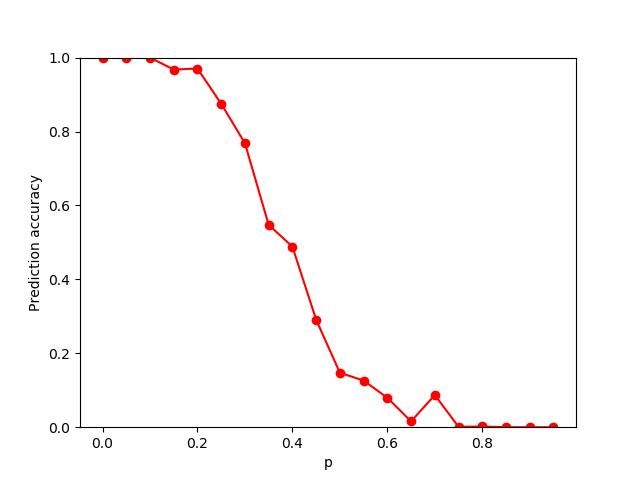
\includegraphics[width=0.75\textwidth]{CompleteGraph_Accuracy_spavg1.png}
\caption{A plot of the data collected using the shortest path metric on the graph constructed from two complete graphs. The graph was constructed using two 200-vertex complete graphs and the probability $q$ of removing edges was set constant at $0.6$.}
\label{fig:complete_graph_plot_shortest_path}
\end{figure}

\begin{figure}[h]
\centering
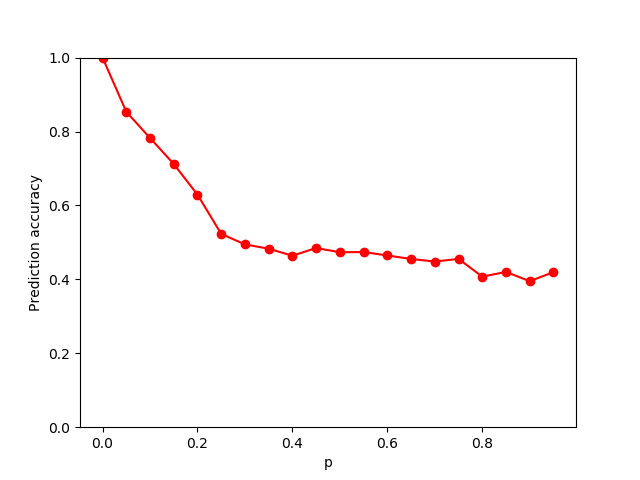
\includegraphics[width=0.75\textwidth]{CompleteGraph_Accuracy_dsdavg1.png}
\caption{A plot of the data collected using the DSD metric on the graph constructed from two complete graphs. The graph was constructed using two 200-vertex complete graphs and the probability $q$ of removing edges was set constant at $0.6$.}
\label{fig:complete_graph_plot_dsd}
\end{figure}

\subsection{Analysis}
\noindent
We do not expect the DSD to do significantly better than the shortest path distance for $p$ from $0$ to $0.5$, as shown in Figure \ref{fig:complete_graph_plot_dsd} and Figure \ref{fig:complete_graph_plot_shortest_path}. This happens because with low probability $p$ of adding edges between components, it is likely that most neighbors of vertices will be within the same component. For example, with probability $p = 0.1$,  there will be significantly fewer edges between the two components compared to edges within each component. This will cause the shortest path metric to predict correctly with a high accuracy since most neighbors of vertices a short distance away will be vertices in the same component. The DSD metric will also predict well since most neighbors of neighbors of a vertex will also be within the same component.

For probability $p$ greater than $0.5$, we expect the DSD metric to outperform the shortest path metric. This is intuitive since with probability of adding edges between components greater than $0.5$, we expect vertices from one component to have more neighbors from the other component than neighbors from the same component. This means that for the shortest path metric, most neighbors a short distance away will have the opposite label. For the DSD metric, however, neighbors of neighbors become equally likely to belong to either component, so the prediction accuracy stays around $50\%$. This clearly shows that the DSD metric considers different aspects of graph structure that the shortest path metric fails to consider.


